\documentclass[a4paper]{article}

% Basic packages
\usepackage{fontspec}
\XeTeXlinebreaklocale "zh"    % 启用中文断行（XeTeX 内建，无需 xeCJK）
\XeTeXlinebreakskip = 0pt plus 1pt
\setmainfont{Songti SC}
\setsansfont{Heiti SC}
\setmonofont{Menlo}
\usepackage{amsmath, amssymb}
\usepackage{graphicx}
\usepackage[margin=2.5cm]{geometry}
\usepackage[most]{tcolorbox}
\usepackage{etoolbox}
\usepackage{listings}
\usepackage{hyperref}
\usepackage{booktabs}
\usepackage{subcaption}
\usepackage{float}

% Chinese font setup (macOS system fonts, no ctex needed)
\setmainfont{Songti SC}
\setsansfont{Heiti SC}
\setmonofont{Menlo}
\newcommand{\song}{\fontspec{Songti SC}}
\newcommand{\hei}{\fontspec{Heiti SC}}
\newcommand{\kai}{\fontspec{KaiTi}}
\newcommand{\fangsong}{\fontspec{FangSong}}

% ===== Highlight boxes =====
\newtcolorbox{knowledgebox}[1]{
    enhanced, colback=blue!5!white, colframe=blue!75!black, colbacktitle=blue!75!black,
    coltitle=white, fonttitle=\bfseries, title=#1, attach boxed title to top left={yshift=-2mm, xshift=2mm},
    boxrule=1pt, sharp corners
}

\newtcolorbox{importantbox}[1]{
    enhanced, colback=yellow!10!white, colframe=yellow!80!black, colbacktitle=yellow!80!black,
    coltitle=black, fonttitle=\bfseries, title=#1, sharp corners
}

\newtcolorbox{warningbox}[1]{
    enhanced, colback=red!5!white, colframe=red!75!black, colbacktitle=red!75!black,
    coltitle=white, fonttitle=\bfseries, title=#1, sharp corners
}

\newtcolorbox{practicebox}[1]{
    enhanced, colback=green!5!white, colframe=green!60!black, colbacktitle=green!60!black,
    coltitle=white, fonttitle=\bfseries, title=#1, sharp corners
}

% ===== Code listings =====
\lstset{
    basicstyle=\ttfamily\small,
    keywordstyle=\color{blue},
    stringstyle=\color{red!60!black},
    commentstyle=\color{green!60!black},
    breaklines=true,
    frame=single,
    numbers=left,
    numberstyle=\tiny\color{gray},
    captionpos=b,
    extendedchars=false
}

% ===== Front-page metadata =====
\newcommand{\notetitle}{CS336 Lecture 16：对齐与强化学习（一）}
\newcommand{\notesubtitle}{Stanford CS336: Language Modeling from Scratch（RLHF、PPO、GRPO 与推理模型）}
\newcommand{\noteauthors}{讲师：Tatsu Hashimoto \quad 笔记：ZCode}
\newcommand{\notedate}{2026-07-14}
\newcommand{\videochannel}{Stanford CS336}
\newcommand{\videopublishdate}{2025 Spring}
\newcommand{\videoduration}{80 分钟}
\newcommand{\videourl}{https://www.youtube.com/watch?v=46f2QTDB08Q}
\newcommand{\videocoverpath}{cover.jpg}

\begin{document}

% ===== Title page =====
\begin{titlepage}
\centering
{\Large 课程笔记\par}
\vspace{1.2cm}
{\huge\bfseries \notetitle\par}
\vspace{0.3cm}
{\large \notesubtitle\par}
\vspace{0.5cm}
{\large \noteauthors\par}
\vspace{0.3cm}
{\large \notedate\par}
\vspace{1.0cm}

\includegraphics[width=0.82\textwidth,height=0.40\textheight,keepaspectratio]{\videocoverpath}\par

\vfill
\begin{tcolorbox}[width=0.9\textwidth, colback=black!2!white, colframe=black!60, sharp corners]
\textbf{视频作者/频道}：\videochannel\par
\textbf{发布日期}：\videopublishdate\par
\textbf{视频时长}：\videoduration\par
\textbf{视频链接}：\href{\videourl}{\nolinkurl{\videourl}}
\end{tcolorbox}
\end{titlepage}

\tableofcontents
\newpage

%% --- 正文内容开始 ---

\section{导论：从 RLHF 到 RLVR}

本讲是后训练（post-training）系列的两讲之二。上一讲围绕 RLHF 与 DPO 展开，本讲首先快速补完 RLHF 的最后几页内容，然后转向近半年最激动人心的方向——\textbf{可验证奖励的强化学习（RL from Verifiable Rewards, RLVR）}，它驱动了当前所有主流推理模型（reasoning models）的训练。

\begin{importantbox}{本讲的双主线}
\textbf{第一部分（算法）}：先把 PPO 讲清楚（上一讲因时长略过的内容），再把 PPO 逐步变形为 GRPO，并深入讨论 GRPO 的实现细节、变体与批评。

\textbf{第二部分（案例研究）}：用三篇代表性的推理模型论文——DeepSeek-R1、Kimi K1.5、Qwen3——展示这些算法在真实工程中如何落地。学完第一部分你就掌握了理解第二部分所需的全部工具。
\end{importantbox}

\section{RLHF 回顾与收尾}

\subsection{DPO 目标与梯度更新}

RLHF 的设定是：我们观察到\textbf{成对偏好数据}（pair-wise preferences，即两个回答中哪个更好），希望学到一个语言模型策略 $\pi_\theta$，使其最大化某种底层奖励在该偏好数据上的期望。难点在于策略 $\pi_\theta$ 出现在期望的"底部"——你是从语言模型中采样的，而不仅仅是最大化似然。

DPO（Direct Preference Optimization）的核心推导是：先做非参数假设（策略类是所有函数的集合），把奖励重写为策略之比，再代入 Bradley-Terry 目标，于是问题被改写为在一种替代参数化下的\textbf{监督学习}。

\begin{figure}[H]
\centering
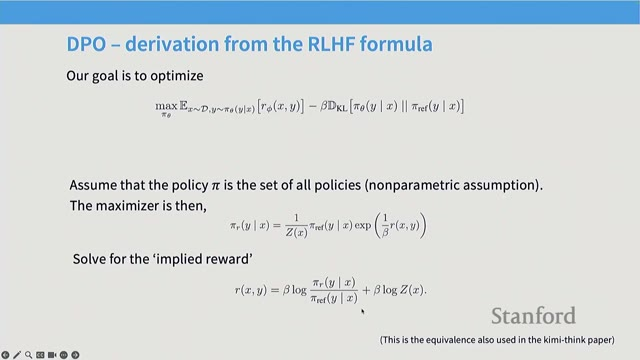
\includegraphics[width=\textwidth]{figures/fig_01_dpo_recap.jpg}
\caption{DPO 的目标函数与梯度更新形式\protect\footnotemark}
\end{figure}
\footnotetext{视频画面时间区间：00:01:30--00:02:10。}

DPO 的梯度更新可以写成非常简洁的形式。参数 $\beta$ 起正则化作用，当奖励估计错误时（隐含奖励不准）更新幅度更大；最终效果就是\textbf{提高好样本的似然、降低坏样本的似然}。

DPO 的核心是非参数假设——把隐含奖励写为策略之比，再代入 Bradley-Terry 目标：

\[
r_\theta(x, y) = \beta \log \frac{\pi_\theta(y|x)}{\pi_{\text{ref}}(y|x)} + \beta \log Z(x)
\]

\begin{itemize}
\item $r_\theta$：由策略隐式定义的奖励
\item $\pi_{\text{ref}}$：参考策略（通常是 SFT 模型），起锚定作用
\item $Z(x)$：与 $y$ 无关的配分函数（partition function），在 Bradley-Terry 中被消去
\end{itemize}

代入成对偏好 $y_w \succ y_l$（$w$ 为偏好项，$l$ 为非偏好项）后得到 DPO 损失：

\[
\mathcal{L}_{\text{DPO}}(\theta) = -\log \sigma\!\left( \beta \log \frac{\pi_\theta(y_w|x)}{\pi_{\text{ref}}(y_w|x)} - \beta \log \frac{\pi_\theta(y_l|x)}{\pi_{\text{ref}}(y_l|x)} \right)
\]

\begin{itemize}
\item $\sigma$：sigmoid 函数
\item $y_w, y_l$：偏好对中的胜者与败者
\item $\beta$：控制偏离参考策略的强度（KL 正则化系数）
\item 该损失是纯监督学习——只需成对偏好数据，无需在线 rollout
\end{itemize}

\begin{knowledgebox}{一句话总结 RL 算法的本质}
几乎所有 RL 算法最终都可以概括为：\textbf{上调好东西、下调坏东西（upweight the good, downweight the bad）}。真正的微妙之处只在于两件事——（1）什么是"好东西"，（2）该上调多少。DPO 只是众多选择中的一种。
\end{knowledgebox}

\subsection{DPO 的变体：SimPO 与长度归一化}

DPO 一度统治了开放模型的后训练流程，因为它比 PPO 容易调通得多。随后出现了 DPO 变体的"论文洪水"——各种 `*PO`。本讲只提两个近期被前沿团队实际采用的：

\begin{tabular}{p{3cm}p{10cm}}
\toprule
\textbf{变体} & \textbf{关键改动} \\
\midrule
SimPO & （1）按回答长度对更新幅度归一化；（2）去掉参考策略 $\pi_{\text{ref}}$ \\
长度归一化 DPO & 保留参考策略，仅按长度归一化 \\
\bottomrule
\end{tabular}

SimPO 去掉参考策略后，就失去了 DPO"策略之比"的数学论证，变成更纯粹的"上调好/下调坏"。其损失按回答长度归一化：

\[
\mathcal{L}_{\text{SimPO}}(\theta) = -\log \sigma\!\left( \frac{\beta}{|y_w|} \log \pi_\theta(y_w|x) - \frac{\beta}{|y_l|} \log \pi_\theta(y_l|x) - \gamma \right)
\]

\begin{itemize}
\item 除以 $|y_w|$、$|y_l|$：按回答长度归一化，避免长回答被系统性惩罚/奖励
\item 无 $\pi_{\text{ref}}$：直接用策略自身的对数似然
\item $\gamma$：额外的 margin 项（目标边距）
\end{itemize}

Tulu 3（AI2）在大量实验中尝试了长度归一化 DPO 和 SimPO，发现它们在某些设置下确实有效。

\begin{warningbox}{RL 的结论高度依赖设置}
RL 的实证结论非常依赖具体条件：基座模型、偏好数据、训练环境、SFT 的质量都会显著改变结论。例如 AI2 早期论文发现 PPO 优于 DPO，但在 Tulu 3 中，只要 SFT 做得更精细，PPO 和 DPO 的增益都会被吃掉，只剩长度归一化 DPO 略胜一筹。\textbf{不要把任何单一实验结果当作普适真理}。
\end{warningbox}

\subsection{过度优化（Overoptimization）}

过度优化是 RLHF 中最核心、最普遍的问题。本质上它就是"高级版的过拟合"，但这个名字之所以重要，是因为它刻画的现象非常危险。

\begin{figure}[H]
\centering
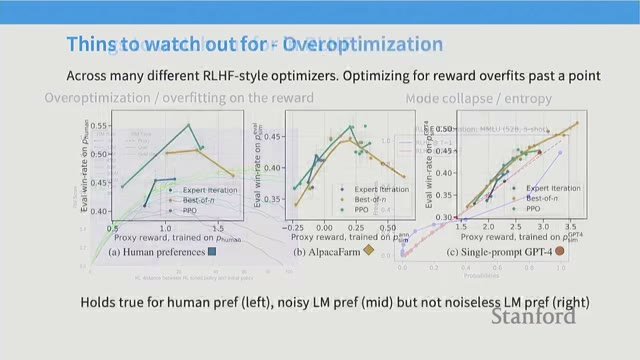
\includegraphics[width=\textwidth]{figures/fig_02_overoptimization.jpg}
\caption{过度优化：代理奖励持续上升，真实偏好却先升后降\protect\footnotemark}
\end{figure}
\footnotetext{视频画面时间区间：00:07:00--00:07:40。}

\textbf{x 轴}是代理奖励（proxy reward，即你拟合的奖励分类器/模型的得分），\textbf{y 轴}是真实偏好胜率（由人类投票或独立的 AI 评测衡量）。一开始两者同向上升，但当代理奖励被优化到一定程度后，真实偏好开始\textbf{下降}——你拟合的奖励模型已经与真实人类偏好发生了分歧。

\begin{itemize}
\item $r_{\text{proxy}}$：在偏好训练集上拟合得到的奖励模型
\item $r_{\text{true}}$：来自真实人类反馈的"上帝视角"奖励
\item 两者\textbf{在期望上}度量同一件事，但在\textbf{有限样本}上不一致——这正是机器学习中训练/测试误差鸿沟的翻版
\end{itemize}

Tatsu 的学生曾做过一项研究：分别用人类偏好、带噪 AI 反馈、无噪 AI 反馈做 RLHF。结果在人类偏好和带噪 AI 反馈上都观察到明显的过度优化曲线，但在无噪 AI 反馈上几乎不出现。这说明\textbf{过度优化主要源于偏好数据的噪声与复杂性}。

\begin{importantbox}{过度优化的工程含义}
做后训练时必须预期：随着代理奖励上升，真实质量并不单调上升。需要设置独立验证信号（如 held-out 偏好、人工 spot-check）来判断何时停止，否则模型会"优化到一个错误的方向上"。
\end{importantbox}

\subsection{RLHF 破坏了模型的校准}

另一个重要的副效应是\textbf{校准（calibration）变差}。在预训练和 SFT 阶段，我们做的是概率建模，模型在某种程度上是"校准的"。但 RLHF 后模型只剩"策略"语义，背后不再有清晰的概率分布。

\begin{figure}[H]
\centering
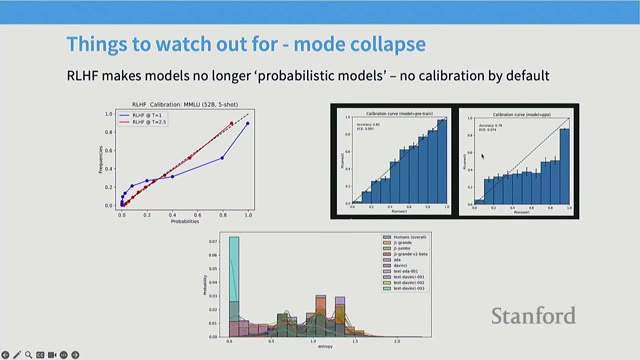
\includegraphics[width=\textwidth]{figures/fig_03_calibration.jpg}
\caption{RLHF 后模型在温度 1 下表现出更强的过度自信\protect\footnotemark}
\end{figure}
\footnotetext{视频画面时间区间：00:08:30--00:09:00。}

来自 Anthropic、GPT-4 发布以及 Tatsu 组的多篇论文都一致显示：RLHF 模型（尤其在温度 1 下）显著\textbf{过度自信}（overconfident）。如果校准本身不在奖励函数里，模型当然没有理由维持校准——这是"按设计"的结果。

\begin{warningbox}{不要把 RLHF 模型当作校准的概率模型}
如果你从生成式建模的背景切入，很容易下意识地把 RLHF 模型当作校准的概率预测器。这是危险的。RLHF 改变了输出分布的形状，使得置信度不再可靠地反映真实不确定性。
\end{warningbox}

\subsection{本章小结}

RLHF 通过 DPO/SimPO 等算法实现了"上调好/下调坏"，但存在两大顽疾：（1）过度优化让代理奖励与真实偏好的关系非单调；（2）破坏概率校准。这些困难正是转向 RLVR 的根本动机。

\section{RLVR：可验证奖励的强化学习}

\subsection{为什么需要 RLVR}

人类反馈存在三重困难：\textbf{容易被 reward hacking}、\textbf{难以大规模采集}、\textbf{难以大规模 RL}。过度优化等问题的根源正在于此。

而 RL 真正取得压倒性胜利的领域是 AlphaGo、AlphaFold——这些领域我们\textbf{知道真实奖励，并能快速、高效、大规模地评估它}。如果能找到这样的领域并把 RL 引入语言建模，就能复用 RL 几十年的成功。

\begin{figure}[H]
\centering
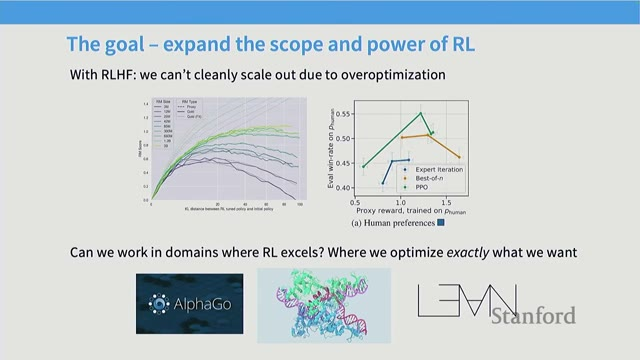
\includegraphics[width=\textwidth]{figures/fig_04_rlvr_motivation.jpg}
\caption{从 RLHF（人类偏好）到 RLVR（可验证奖励）的范式转移\protect\footnotemark}
\end{figure}
\footnotetext{视频画面时间区间：00:12:55--00:13:25。}

\begin{knowledgebox}{RLHF 与 RLVR 的对照}
RLHF：奖励来自人类偏好（噪声大、难采集、易被 hack、导致过度优化）。
RLVR：奖励来自可程序化验证的真值（数学答案对错、代码测试通过），干净、可大规模评估、几乎不可能被 reward hacking。范式从"讨好人类"转向"解对题目"。
\end{knowledgebox}

\begin{importantbox}{RLVR 的核心心法}
与其用"用户是否喜欢这个机器人"这一难优化、易被 hack 的目标，不如\textbf{选择一个我们知道真实奖励、且能高效评估的领域}（如数学：答案对就是对、错就是错），然后把 RL 的全部武器搬过来。这正是从 ChatGPT-3.5 时代迈向 o1 时代的关键思路转变。
\end{importantbox}

\subsection{本讲地图}

\begin{tabular}{p{3cm}p{10cm}}
\toprule
\textbf{部分} & \textbf{内容} \\
\midrule
第一部分 & PPO（详细）$\to$ GRPO（简化）$\to$ GRPO 变体与 Dr.GRPO 批评 \\
第二部分 & DeepSeek-R1（R1-Zero、R1）、Kimi K1.5、Qwen3 三个案例研究 \\
\bottomrule
\end{tabular}

\section{策略梯度与 PPO}

\subsection{从最简单的策略梯度开始}

理解 PPO 的最佳路径是从最简单的东西出发，再一步步往下走。最简单的就是\textbf{策略梯度（policy gradient）}：在当前策略 $\pi_\theta$ 下最大化期望奖励，对其求梯度可得：

\begin{figure}[H]
\centering
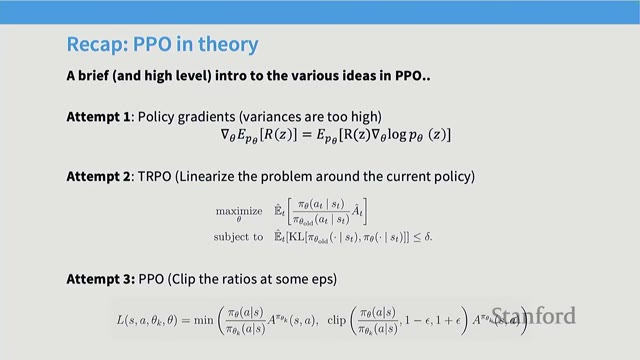
\includegraphics[width=\textwidth]{figures/fig_05_policy_gradient.jpg}
\caption{策略梯度：期望奖励对参数求梯度\protect\footnotemark}
\end{figure}
\footnotetext{视频画面时间区间：00:15:00--00:15:30。}

\[
\nabla_\theta J(\theta) = \mathbb{E}_{z \sim \pi_\theta}\left[ r(z)\, \nabla_\theta \log \pi_\theta(z) \right]
\]

\begin{itemize}
\item $z$：从策略 $\pi_\theta$ 采样的一条轨迹（rollout）
\item $r(z)$：该轨迹的奖励
\item $\nabla_\theta \log \pi_\theta(z)$：对数似然的得分函数（score function）
\item 根据奖励的符号，梯度会相应地\textbf{提高或降低}该样本的概率
\end{itemize}

策略梯度的两个低效之处：第一，它是\textbf{纯 on-policy} 的——每次梯度步都要从 $\pi_\theta$ 重新采样并立即更新；第二，RL 最贵的部分是 rollout（运行语言模型生成样本），而 on-policy 不允许我们对同一批样本多次更新。

更根本地，我们想要最大化的原始目标是策略下的期望奖励：

\[
J(\theta) = \mathbb{E}_{z \sim \pi_\theta}\left[ r(z) \right]
\]

\begin{itemize}
\item $\pi_\theta$：参数为 $\theta$ 的策略（语言模型）
\item $r(z)$：轨迹 $z$ 的奖励
\item 这是一个\textbf{策略上的期望}——策略本身既是被优化的对象，又出现在期望的分布中，这正是它难于优化的原因
\end{itemize}

\subsection{TRPO：重要性采样修正}

为了减少采样次数，希望允许"更新变旧"——从旧的 $\pi_{\theta_{\text{old}}}$ 采样、做多次更新，但仍保持策略梯度的有效性。做法是\textbf{重要性采样（importance sampling）修正}，并用 KL 约束把新策略限制在旧策略附近，避免奖励估计失真。

\begin{figure}[H]
\centering
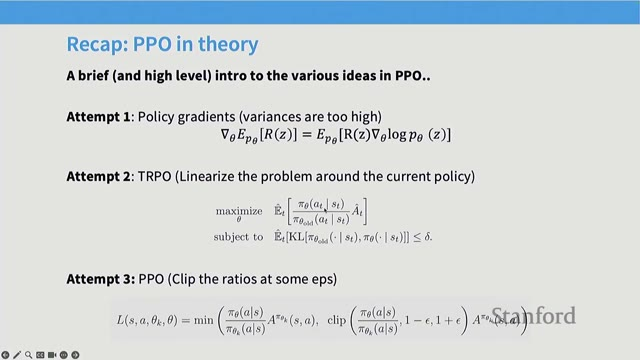
\includegraphics[width=\textwidth]{figures/fig_06_trpo.jpg}
\caption{TRPO：重要性采样 + KL 约束，允许 off-policy 更新\protect\footnotemark}
\end{figure}
\footnotetext{视频画面时间区间：00:16:35--00:17:00。}

\[
\nabla_\theta J(\theta) = \mathbb{E}_{z \sim \pi_{\theta_{\text{old}}}}\left[ \frac{\pi_\theta(z)}{\pi_{\theta_{\text{old}}}(z)}\, A(z)\, \nabla_\theta \log \pi_\theta(z) \right]
\]

\begin{itemize}
\item $\frac{\pi_\theta(z)}{\pi_{\theta_{\text{old}}}(z)}$：重要性采样比，修正分布偏移
\item $A(z)$：优势函数（advantage），是 $r(z)$ 的低方差版本
\item TRPO 用\textbf{KL 散度硬约束}保证 $\pi_\theta \approx \pi_{\theta_{\text{old}}}$
\end{itemize}

\subsection{PPO：用 clip 代替 KL}

PPO 是在 TRPO 之上再走一步：\textbf{不做 KL 散度，而是直接截断（clip）优势函数}。当策略偏离过远时，奖励会被截断在 $1-\varepsilon$ 或 $1+\varepsilon$ 处，RL 算法再没有动机让策略跑得更远——这是一种软约束。

\begin{figure}[H]
\centering
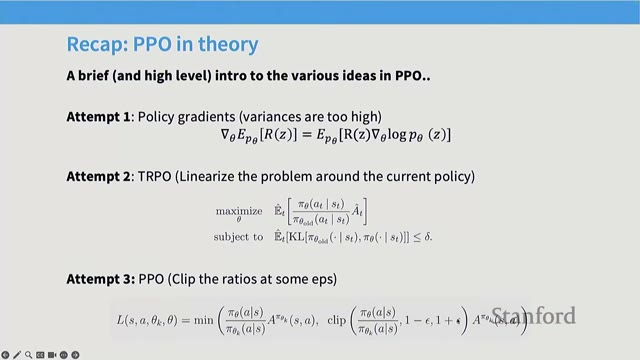
\includegraphics[width=\textwidth]{figures/fig_07_ppo_clip.jpg}
\caption{PPO clip 目标：截断重要性比，自然约束策略漂移\protect\footnotemark}
\end{figure}
\footnotetext{视频画面时间区间：00:17:15--00:17:35。}

\[
L^{\text{CLIP}}(\theta) = \mathbb{E}\left[ \min\left( \rho_t(\theta)\, A_t,\; \text{clip}(\rho_t(\theta),\, 1-\varepsilon,\, 1+\varepsilon)\, A_t \right) \right]
\]

\begin{itemize}
\item $\rho_t(\theta) = \pi_\theta(a_t|s_t) / \pi_{\theta_{\text{old}}}(a_t|s_t)$：重要性比
\item $\varepsilon$：截断范围，典型值 $0.2$，即允许的似然比区间为 $[0.8, 1.2]$
\item $A_t$：优势函数，由\textbf{价值函数（value function）}计算，用于方差缩减
\end{itemize}

\begin{importantbox}{PPO 需要第二个神经网络}
PPO 的优势 $A_t$ 需要一个\textbf{价值网络}来估计期望回报以降低梯度方差。这个价值网络通常和策略网络一样大——这意味着\textbf{GPU 显存翻倍}。这是后来 GRPO 试图摆脱 PPO 的核心动机之一。
\end{importantbox}

\subsection{PPO 的工程实现：一个"巨兽"}

PPO 在概念上不复杂，但工程上极其繁琐。有一篇著名的博客《37 implementation details of PPO》以及专门论文论证"实现细节比算法本身更重要"——甚至有些细节严格意义上\textbf{违反了策略梯度推导，却反而效果更好}。

\begin{figure}[H]
\centering
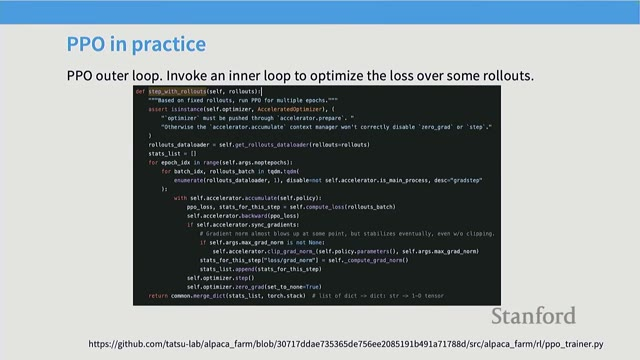
\includegraphics[width=\textwidth]{figures/fig_08_ppo_implementation.jpg}
\caption{早期 RLHF 的 PPO 实现示意图：奖励模型、价值模型、GAE 一应俱全\protect\footnotemark}
\end{figure}
\footnotetext{视频画面时间区间：00:20:30--00:21:30。}

标准 PPO 实现包含以下组件：

\begin{tabular}{p{2.8cm}p{4cm}p{6.5cm}}
\toprule
\textbf{组件} & \textbf{作用} & \textbf{实现要点} \\
\midrule
外层训练循环 & 标准 LM 梯度更新 & rollout $\to$ 算 loss $\to$ backward + grad clip \\
价值函数 loss & 拟合期望回报 & 与策略同步更新 \\
PPO clip loss & 截断重要性比 & $\varepsilon=0.2$ \\
rollout 模块 & 采样 + 算 logprob & 价值/奖励/策略分词器不同需重分词 \\
reward shaping & 构造 per-token 奖励 & KL 按 token、真奖励只在终止 token \\
GAE & 方差缩减 & 可设 $\gamma=\lambda=1$ 退化为 baselined PG \\
\bottomrule
\end{tabular}

\subsection{上下文老虎机与奖励整形}

一个关键观察：语言模型的 RL 在某种意义上是\textbf{上下文老虎机（contextual bandit）}——给定 prompt 生成一个回答，立即获得奖励，没有状态转移、没有环境探索。这种结构使得奖励可以这样塑造：

\begin{itemize}
\item \textbf{终止奖励（terminal reward）}：任务是否成功（如数学答案对错），只在最后一个 token 上给出
\item \textbf{per-token 奖励}：KL 正则项按 token 计算，作为"持续的小惩罚"
\end{itemize}

\begin{knowledgebox}{KL 的实现细节陷阱}
PPO 实现中常按 token 加 KL 惩罚，但代码中往往把 log-似然比在为负时\textbf{截断到 0}以避免数值不稳定——这其实已经不再是严格意义的 KL 了，而是一种近似。这种"工程近似"在 RLHF 代码中非常普遍。
\end{knowledgebox}

更精确地说，per-token 的 KL 惩罚项形如：

\[
\hat{D}_{\text{KL}}\left( \pi_\theta \| \pi_{\text{ref}} \right) = \frac{\pi_{\text{ref}}(o_t|s_t)}{\pi_\theta(o_t|s_t)} - \log \frac{\pi_{\text{ref}}(o_t|s_t)}{\pi_\theta(o_t|s_t)} - 1
\]

该 per-token 惩罚在所有非终止 token 上累加，而\textbf{任务奖励（如答案对错）只在最后一个 token 上给出}：

\[
R_{\text{total}}(z) = \mathbb{1}[\text{correct}] + \sum_{t=1}^{|z|} \beta \cdot \hat{D}_{\text{KL}}^{(t)}
\]

\subsection{广义优势估计（GAE）}

策略梯度的方差通常很高，需要尽可能的方差缩减。与其直接用 $r(z)$ 乘梯度，可以用一个\textbf{折扣优势估计} $A_t$ 替代，其形式由 GAE（Generalized Advantage Estimation）给出：

\begin{figure}[H]
\centering
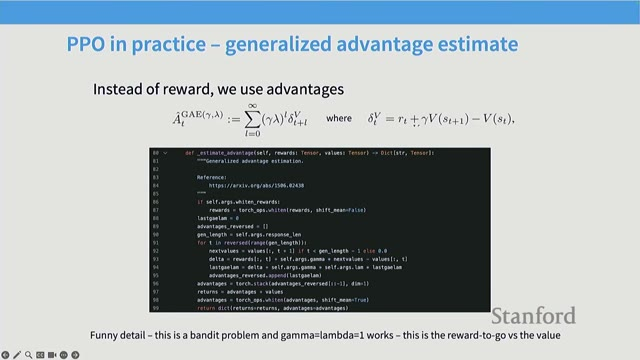
\includegraphics[width=\textwidth]{figures/fig_09_gae.jpg}
\caption{GAE：通过 $\gamma$、$\lambda$ 在偏差与方差间权衡\protect\footnotemark}
\end{figure}
\footnotetext{视频画面时间区间：00:26:15--00:26:45。}

\[
A_t = \sum_{l=0}^{\infty} (\gamma \lambda)^l\, \delta_{t+l}, \quad \delta_t = r_t + \gamma V(s_{t+1}) - V(s_t)
\]

\begin{itemize}
\item $\delta_t$：时序差分（TD）误差
\item $\gamma$：折扣因子，控制对未来回报的重视
\item $\lambda$：GAE 参数，在偏差（$\lambda \to 0$）与方差（$\lambda \to 1$）间权衡
\item $V(s)$：价值函数估计
\item 一个有趣的事实：取 $\gamma = \lambda = 1$，GAE 退化为\textbf{baselined 策略梯度}（$R - V$），往往也能很好地工作
\end{itemize}

\subsection{本章小结}

PPO = 策略梯度 + 重要性采样修正 + clip 软约束 + 价值函数 + GAE。它在通用 RL 上极其成功（OpenAI 的 Dota 机器人、各种 toy 环境），但在语言模型上是一个"巨兽"——37 个实现细节、需要与策略等大的价值网络、容易翻车的 KL 近似。这正是后续寻找替代方案的动机。

\section{GRPO：去掉价值模型的简化方案}

\subsection{GRPO 的核心思路}

人们想要：能像 PPO 那样适用通用 RL 设置、但\textbf{不要复杂的实现}、更重要的\textbf{不要价值模型}的算法。DPO 不合适——它针对成对 Bradley-Terry 偏好，不适合"数学答案对错"这种无成对结构的场景；它本质上是离线算法。

于是就有了 GRPO（Group Relative Policy Optimization）。GRPO 极其简单：从 PPO 出发，保留 clip 与策略更新的思想，但\textbf{彻底删掉 GAE}，换成一个简单得多的优势估计。

\begin{figure}[H]
\centering
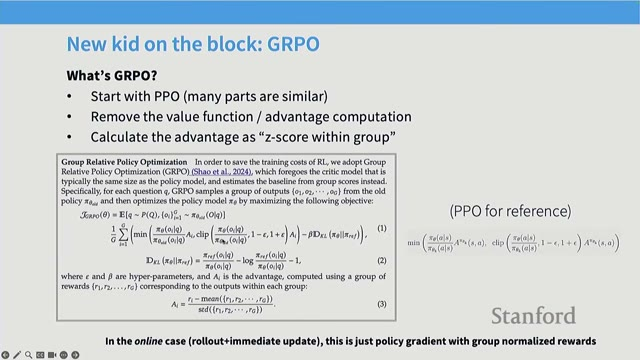
\includegraphics[width=\textwidth]{figures/fig_10_grpo_intro.jpg}
\caption{GRPO：用组内 z-score 替代 GAE，去掉价值模型\protect\footnotemark}
\end{figure}
\footnotetext{视频画面时间区间：00:29:25--00:29:55。}

\subsection{组内 z-score 优势}

\begin{figure}[H]
\centering
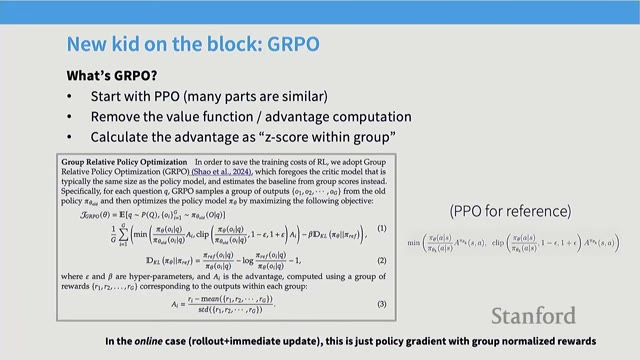
\includegraphics[width=\textwidth]{figures/fig_11_grpo_group.jpg}
\caption{GRPO 的组（group）：同一问题的 $G$ 个候选回答\protect\footnotemark}
\end{figure}
\footnotetext{视频画面时间区间：00:30:00--00:30:45。}

GRPO 的优势定义为：

\[
A_i = \frac{r_i - \text{mean}(r_1, \dots, r_G)}{\text{std}(r_1, \dots, r_G)}
\]

\begin{itemize}
\item $r_i$：第 $i$ 个回答的奖励
\item $\text{mean}$、$\text{std}$：\textbf{同一问题}的 $G$ 个回答的组内均值与标准差
\item 这是对组内奖励的\textbf{z-score}（标准化得分）
\item "组"对语言模型 RL 是天然对象：一个输入问题（如一道数学题）+ $G$ 个候选回答构成一组
\end{itemize}

带 clip 的 GRPO 完整目标函数为：

\[
\mathcal{J}_{\text{GRPO}}(\theta) = \mathbb{E}\left[ \frac{1}{G}\sum_{i=1}^{G} \min\!\left( \rho_i A_i,\, \text{clip}(\rho_i, 1-\varepsilon, 1+\varepsilon) A_i \right) - \beta\, \hat{D}_{\text{KL}} \right]
\]

\begin{itemize}
\item $\rho_i = \pi_\theta(o_i|q) / \pi_{\theta_{\text{old}}}(o_i|q)$：重要性采样比
\item $A_i$：组内 z-score 优势
\item $\hat{D}_{\text{KL}}$：策略与参考策略的 KL 估计
\item 与 PPO 相比，只是把价值函数算出的 GAE 换成了组内 z-score
\end{itemize}

baselining 是策略梯度降低方差的核心技巧。经典结果表明，可以减去任意\textbf{不依赖当前样本}的基线 $B$ 而不改变梯度期望：

\[
\nabla_\theta J(\theta) = \mathbb{E}_{z \sim \pi_\theta}\left[ \left( r(z) - B \right) \nabla_\theta \log \pi_\theta(z) \right]
\]

\begin{itemize}
\item $B$：基线，只要与 $z$ 独立（或为常数），在策略上求和为 0
\item 减去合适的 $B$ 可\textbf{大幅降低梯度方差}而不引入偏差
\item GRPO 的组内均值正是这样一种自适应基线
\end{itemize}

\begin{knowledgebox}{"组"的工程含义}
在工程实现中，你会同时处理多个问题，每个问题采样 $G$ 个回答构成一组；baseline 只在\textbf{组内}做（同一问题的 $G$ 个回答之间归一化），跨问题之间不做 baselining，只共享策略更新。这种结构天然适配 batch 训练——一个 batch 由若干个"问题 $\times$ $G$ 回答"的组拼成。
\end{knowledgebox}

\begin{importantbox}{为什么组内 baseline 是合理的}
不同问题的难度不同——简单的题平均奖励高、难题平均奖励低。组内均值天然捕捉了"问题难度"，作为每个样本自身的\textbf{基线（baseline）}被减掉。这正是"policy gradient with leave-one-out baseline"思想的简化（去掉标准差项即为 leave-one-out）。\textbf{baseline 只在同一个问题内部做}，跨问题不做 baselining，只共享策略更新。
\end{importantbox}

\subsection{纯在线情形的极简形式}

如果只做一步纯在线更新（即不重复使用 rollout），所有的 clip 机制都可以丢掉，剩下的就是纯粹的策略梯度——\textbf{上调好东西、下调坏东西}，只不过乘上去的权重变成了 $A_i$。这是一个极其简单的算法。

\subsection{KL 散度的控制变量估计}

GRPO 中的 KL 散度 $D_{\text{KL}}$ 估计有点非标准。自然的 KL 估计是对 log 比求平均，但 GRPO 用了带两个额外项的形式：

\begin{figure}[H]
\centering
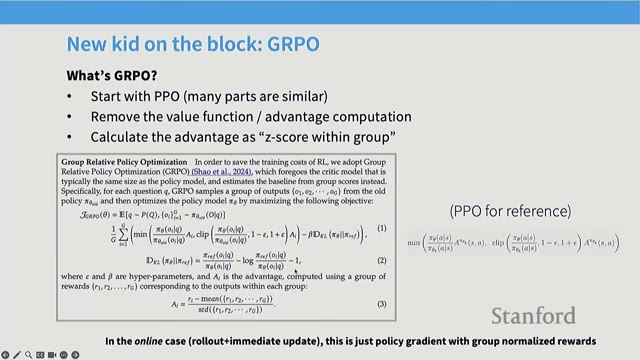
\includegraphics[width=\textwidth]{figures/fig_12_kl_control_variate.jpg}
\caption{GRPO 的 KL 估计：控制变量（control variate）方案以降低方差\protect\footnotemark}
\end{figure}
\footnotetext{视频画面时间区间：00:32:45--00:33:15。}

\[
D_{\text{KL}} \approx \frac{\pi_{\text{ref}}(o|x)}{\pi_\theta(o|x)} - \log \frac{\pi_{\text{ref}}(o|x)}{\pi_\theta(o|x)} - 1
\]

\begin{itemize}
\item 第一项 $\frac{\pi_{\text{ref}}}{\pi_\theta}$ 在对 $\pi_\theta$ 求期望时与第三项 $-1$ 抵消
\item 这构成一个\textbf{控制变量（control variate）}，在不改变期望的同时降低方差
\item 这是估计 KL 的一个更"漂亮"的方式，值得在需要从样本估计 KL 时借鉴
\end{itemize}

\subsection{GRPO 的实现与超参}

GRPO 的实现几乎逐行对应其公式。外层循环：对每个 rollout 算奖励、组内归一化（均值和方差）、算 KL（实现中按 sequence 算，重型实现会更细）、对 loss 做梯度更新。优势计算几乎逐行照抄公式，唯一的小差异是\textbf{除以标准差时加一个小的 $10^{-4}$ 防 0}：

\[
A_i = \frac{r_i - \bar{r}}{\sqrt{\frac{1}{G}\sum_{j=1}^{G}(r_j - \bar{r})^2} + \epsilon}, \quad \epsilon = 10^{-4}
\]

\begin{itemize}
\item $\bar{r} = \frac{1}{G}\sum_j r_j$：组内均值
\item 分母加 $\epsilon$：防止当组内奖励完全相同（标准差为 0）时除零崩溃
\item 这是几乎所有 RL 归一化代码都会做的标准技巧
\end{itemize}

\begin{practicebox}{作业提示}
在 A5 中你将实现 GRPO。优势计算需要加一个小的 epsilon（如 $10^{-4}$）防止除以 0；KL 在不同实现中可以是 per-token 或 per-sequence；价值/奖励/策略模型若分词器不同需要重分词。
\end{practicebox}

\subsection{DeepSeek-Math 的实证结果}

GRPO 来自 DeepSeek-Math 论文。该论文比较了多种方法：

\begin{figure}[H]
\centering
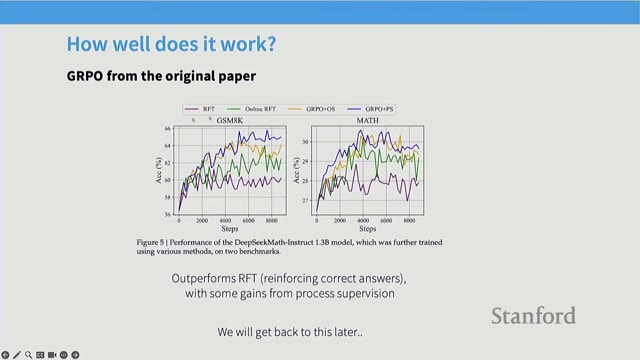
\includegraphics[width=\textwidth]{figures/fig_13_deepseekmath_results.jpg}
\caption{DeepSeek-Math：RFT、GRPO（结果奖励）与 GRPO（过程奖励）对比\protect\footnotemark}
\end{figure}
\footnotetext{视频画面时间区间：00:35:00--00:35:40。}

\begin{itemize}
\item \textbf{RFT/Online RFT}：只对答对的样本做 SFT，是较弱的基线
\item \textbf{GRPO + outcome reward}（黄色）：只用答案对/错的二元奖励
\item \textbf{GRPO + process reward}（蓝色）：对每步推理打分（PRM），论文论证 PRM 更好
\item 结论：GRPO 有效，效果显著
\end{itemize}

\begin{warningbox}{PRM 的"翻转"}
有意思的是：DeepSeek-Math 阶段他们对 PRM 信心满满（蓝线最优），但到了 R1 论文，他们反而放弃了 PRM，回到了\textbf{纯结果奖励}。这一翻转贯穿整个推理模型的发展史，值得反复体会。
\end{warningbox}

\section{Dr.GRPO：对 GRPO 的数学批评}

回到策略梯度定理。一条经典结果是：可以减去任意\textbf{不依赖当前样本}的基线 $B(s)$ 而保持梯度期望不变——因为 $B(s)$ 在策略上求和为 0。这叫做\textbf{baselining}，是降低方差的标准工具。

GRPO 的 $A_i$ 是基线吗？减去组内均值勉强符合（只要不含 $r_i$ 自身），但\textbf{除以标准差}这一步在数学上是有问题的——它不在策略梯度定理所允许的操作内。

\begin{figure}[H]
\centering
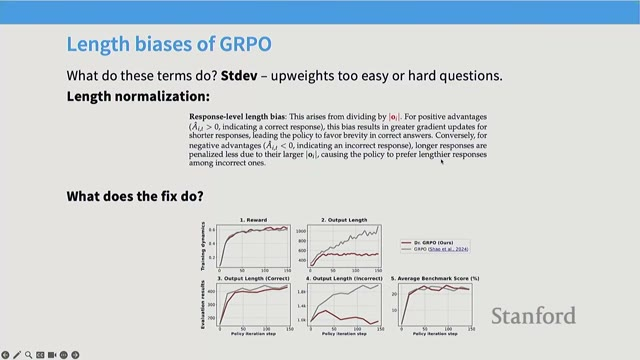
\includegraphics[width=\textwidth]{figures/fig_14_drgrpo_criticism.jpg}
\caption{Dr.GRPO：GRPO 的两个数学"不合规"之处\protect\footnotemark}
\end{figure}
\footnotetext{视频画面时间区间：00:39:25--00:40:00。}

\subsection{偏差一：除以标准差}

当标准差小时（问题太容易，奖励全为 1；或太难，全为 0），优势会被\textbf{放大}——算法会过度优化那些"太容易或太难"的组。这与理想的"课程效应"背道而驰：我们真正想喂给模型的是\textbf{难度适中、能学到东西}的样本。

\begin{importantbox}{folk theorem 的直觉}
RL 算法最想拿到的是"模型有时做对、有时做错"的样本——这样才有学习信号。除以标准差反而把优化压力推向两个极端（要么全对、要么全错），这些样本几乎没有可学的梯度方向，可能拖慢收敛，至少在数学上破坏了策略梯度的有效性。
\end{importantbox}

\subsection{偏差二：长度归一化}

GRPO 还把奖励按输出长度归一化。这看起来无害，却引入了糟糕的激励：

\begin{figure}[H]
\centering
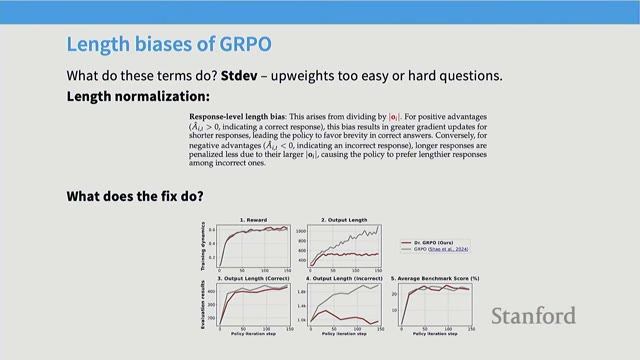
\includegraphics[width=\textwidth]{figures/fig_15_drgrpo_length.jpg}
\caption{Dr.GRPO 修正后：输出长度不再无限增长\protect\footnotemark}
\end{figure}
\footnotetext{视频画面时间区间：00:40:25--00:41:00。}

\begin{itemize}
\item \textbf{答错时}：得到负奖励，最优策略是\textbf{把回答拉到无限长}以稀释负奖励
\item \textbf{答对时}：得到正奖励，最优策略是\textbf{把回答压到最短}以最大化单位长度奖励
\item 结果：模型产生"答错时疯狂胡说、答对时惜字如金"的扭曲激励
\end{itemize}

Dr.GRPO 的作者主张同时去掉这两个偏差。实验显示：在 GSM8K 等 toy 任务上，修正后能达到相同奖励，但\textbf{输出长度不再无限增长}，而是稳定在一个水平。

修正后的 Dr.GRPO 优势定义为：

\[
A_i^{\text{Dr.GRPO}} = r_i - \text{mean}(r_1, \dots, r_G)
\]

\begin{itemize}
\item 去掉了除以标准差，只保留减去均值
\item 这回到了合法的 leave-one-out baseline，符合策略梯度定理的要求
\item 不再过度放大"太易/太难"的样本
\end{itemize}

\begin{knowledgebox}{对"长 CoT 是必然"的质疑}
一个引人深思的假说：我们看到的许多超长思维链（CoT），可能并非推理能力的内在需求，而是\textbf{GRPO 实现细节的副产物}。这一假说虽未完全证实，但 Dr.GRPO 的实验提供了相当有力的旁证。
\end{knowledgebox}

\section{案例研究一：DeepSeek-R1}

R1 是一篇引发社会现象的 arXiv 论文——一度让 Nvidia 蒸发近五亿美元市值。它的贡献在于：用\textbf{极其简单的配方}复现了 OpenAI o1 的全部定性能力。

\begin{itemize}
\item \textbf{性能}：全面逼近 o1
\item \textbf{配方}：没有搜索、没有 PRM、没有花哨的机制——纯 RL
\item \textbf{科学洞见}：SFT 与 RL 之间交互的许多细节
\end{itemize}

\subsection{R1-Zero：纯 RL 的受控实验}

R1-Zero 是 R1 的"研究设置"。它直接拿预训练+mid-trained 的 DeepSeek-V3 基座（不做任何 RLHF 或指令微调），扔进数学 RL 循环。

\begin{figure}[H]
\centering
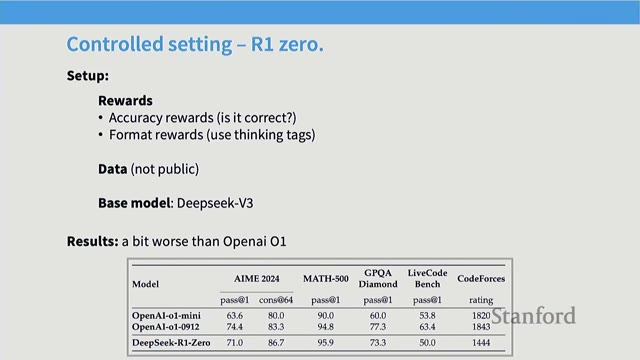
\includegraphics[width=\textwidth]{figures/fig_16_r1_zero.jpg}
\caption{R1-Zero：基座模型直接做 RL，无 SFT\protect\footnotemark}
\end{figure}
\footnotetext{视频画面时间区间：00:46:15--00:46:45。}

\begin{tabular}{p{3cm}p{10cm}}
\toprule
\textbf{要素} & \textbf{设置} \\
\midrule
基座 & DeepSeek-V3（pre-trained + mid-trained） \\
数据 & 类数学任务（数据未公开） \\
奖励 1 & \textbf{accuracy reward}：答案对/错，二元 \\
奖励 2 & \textbf{format reward}：强制把思维链放进 \texttt{<think></think>} 标签 \\
\bottomrule
\end{tabular}

R1-Zero 的总奖励是 accuracy 与 format 两项之和：

\[
R(o, q) = R_{\text{accuracy}}(o, q) + R_{\text{format}}(o)
\]

\begin{itemize}
\item $R_{\text{accuracy}} \in \{0, 1\}$：答案是否正确（由规则判题器或模型判等给出）
\item $R_{\text{format}} \in \{0, 1\}$：回答是否包含合法的 \texttt{<think>}/\texttt{</think>} 标签
\item 这是一种\textbf{纯可验证奖励}——无任何人类偏好参与
\end{itemize}

\begin{importantbox}{format reward 看似无关，实则关键}
format reward 表面是个无关紧要的格式约束，但据许多论文和工程实践反馈：它其实是\textbf{让整套推理 RL 跑通的关键部件}之一。没有它，模型很难稳定地产出可被后续流程利用的长 CoT。
\end{importantbox}

\subsection{"aha moment" 与回溯现象}

R1-Zero 训练中出现两个被大肆宣传的现象：

\begin{figure}[H]
\centering
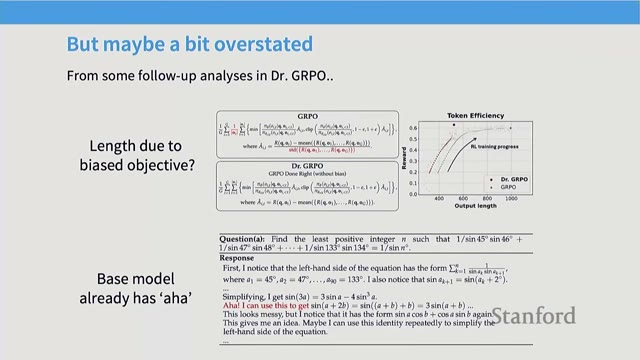
\includegraphics[width=\textwidth]{figures/fig_17_r1_aha_moment.jpg}
\caption{R1-Zero 的"aha moment"：模型自发学会回溯\protect\footnotemark}
\end{figure}
\footnotetext{视频画面时间区间：00:48:30--00:49:00。}

\begin{enumerate}
\item \textbf{CoT 长度随训练稳定增长}——论文浪漫地解读为"模型学会了想得更深来解更难的题"
\item \textbf{涌现出"aha moment"与回溯}——模型会写出"wait, I think I made a mistake..."这样的自我纠正
\end{enumerate}

\begin{warningbox}{Dr.GRPO 的反驳}
Dr.GRPO 作者对这两个现象提出了相当有力的反驳：（1）长度增长可能只是\textbf{有偏目标}的副产物，而非涌现能力；（2）把 DeepSeek-V3 直接跑在数学题上，它也会偶尔输出"aha, I can do this"——这未必是 RL 带来的新现象。近期证据让这些"涌现性"解释变得不再那么可信。
\end{warningbox}

\subsection{R1 的完整流水线}

R1-Zero 是研究设置，要部署一个真正能交付的强模型，需要更完整的流水线。

\begin{figure}[H]
\centering
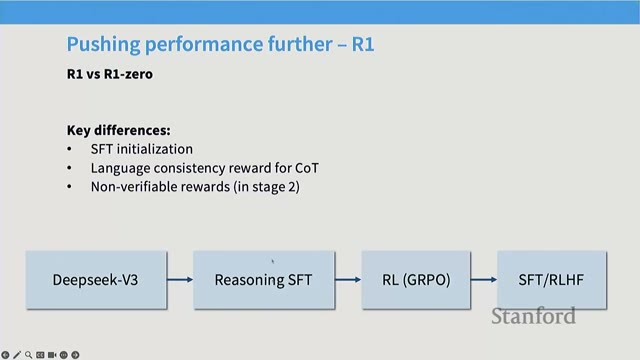
\includegraphics[width=\textwidth]{figures/fig_18_r1_pipeline.jpg}
\caption{R1 完整流水线：长 CoT SFT $\to$ RL $\to$ 二次 SFT $\to$ RLHF\protect\footnotemark}
\end{figure}
\footnotetext{视频画面时间区间：00:50:00--00:50:30。}

\begin{enumerate}
\item \textbf{长 CoT SFT 初始化}：用来源不明的长 CoT 数据做 SFT，让模型先"会"长思维链，再进 RL（论文对数据来源语焉不详）
\item \textbf{推理 RL}：基本同 R1-Zero，额外加\textbf{语言一致性奖励}（language consistency reward），防止 CoT 中途切换语言
\item \textbf{二次 SFT}：把推理数据 + 非推理数据（写作、证明等非可验证任务，用 self-judge）+ DeepSeek-V3 的 SFT 数据合并
\item \textbf{RLHF}：仍用 GRPO 做 RLHF，沿用 V3 的偏好训练流程
\end{enumerate}

\begin{knowledgebox}{语言一致性奖励的必要性}
Tatsu 强调一个有意思的现象：若不加这个奖励，模型在 RL 过程中 CoT 会\textbf{语言混合}——比如突然从英文切到中文（这正是互联网上用户抱怨"Grok 3 突然说中文"的根源）。这表明模型天然有语言混合倾向，需要额外奖励约束。代价是它略微牺牲了性能，但换取了 CoT 的可读性。
\end{knowledgebox}

\subsection{R1 的性能}

\begin{figure}[H]
\centering
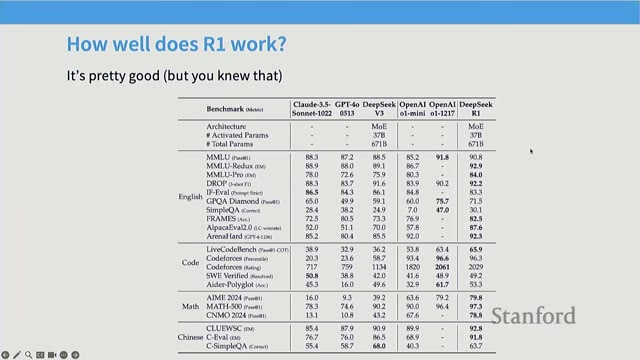
\includegraphics[width=\textwidth]{figures/fig_19_r1_performance.jpg}
\caption{R1 在英文任务上几乎全面匹配 o1\protect\footnotemark}
\end{figure}
\footnotetext{视频画面时间区间：00:54:35--00:54:55。}

R1 的结果震撼了整个社区：英文任务全面匹配 o1，代码略差但非常接近。考虑到其配方的简洁性，这一结果几乎超出所有人的预期。

\subsection{R1 的蒸馏}

\begin{figure}[H]
\centering
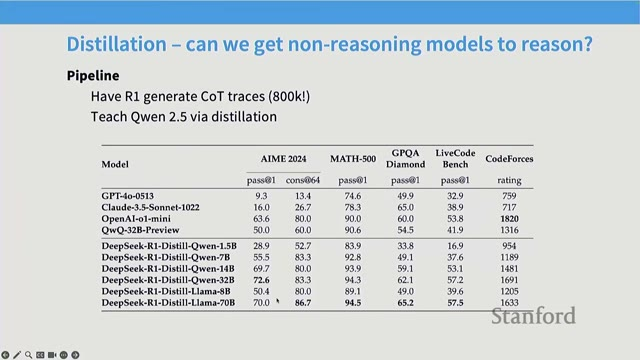
\includegraphics[width=\textwidth]{figures/fig_20_r1_distillation.jpg}
\caption{R1 蒸馏：百万级 CoT 灌给 Qwen，性能大幅提升\protect\footnotemark}
\end{figure}
\footnotetext{视频画面时间区间：00:55:05--00:55:30。}

R1 团队把 R1 生成的近百万条思维链作为 SFT 数据，fine-tune Qwen 等小模型。例如 32B 的 Qwen 基模 AIME 只有约 50\%，蒸馏后能提升 25 个百分点以上。这再次印证：\textbf{长 CoT 能力其实早已"潜伏"在基座里}，只需少量数据就能"激活"。

Tatsu 自己组里也验证过：用 Gemini 2.0 Flash Thinking 的 1000 条长 CoT fine-tune Qwen 2.5，就能获得非常显著的数学 benchmark 提升。

\subsection{R1 的三大科学贡献}

\begin{enumerate}
\item \textbf{正面证据}：纯结果奖励 + GRPO 就能训出强推理模型
\item \textbf{负面结果 1}：PRM 不奏效——他们在 R1 上反复尝试 PRM 都没能复现 o1
\item \textbf{负面结果 2}：基于搜索的方法（MCTS）也没奏效
\end{enumerate}

\begin{importantbox}{两个"不奏效"的意义}
DeepSeek 在 DeepSeek-Math 阶段对 PRM 信心十足（蓝线最优），但到 R1 却回归纯结果奖励；MCTS 等搜索方法也未能跑通。这两个负面结果让"结果奖励 + RL"成为推理模型的最强基线，至今未被撼动。
\end{importantbox}

\section{案例研究二：Kimi K1.5}

Kimi K1.5 与 R1 几乎同期发布，达成了非常接近的结果，但用了\textbf{不同的算法和工程细节}。两者构成"趋同演化（convergent evolution）"——同一问题被两条路径独立攻下，对照阅读价值极高。

\subsection{数据构造}

\begin{figure}[H]
\centering
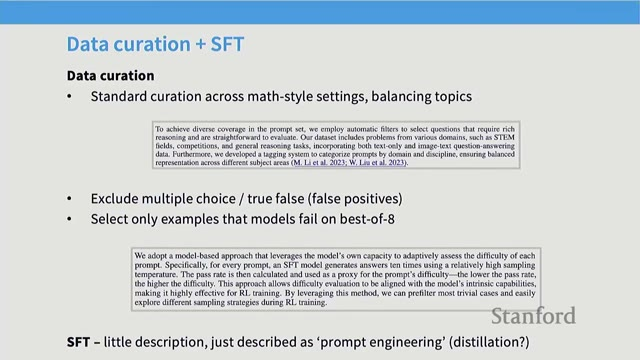
\includegraphics[width=\textwidth]{figures/fig_21_kimi_data.jpg}
\caption{Kimi K1.5 数据：best-of-8 难度过滤 + 域平衡\protect\footnotemark}
\end{figure}
\footnotetext{视频画面时间区间：01:01:55--01:02:25。}

\begin{tabular}{p{3.5cm}p{9.5cm}}
\toprule
\textbf{策略} & \textbf{做法} \\
\midrule
域平衡 & 用 LM 自动给数学题打学科标签，跨学科平衡保证多样性 \\
排除 MCQ/判断题 & 太容易被 hack 或随机猜对，只保留可用 regex/LM 评判的短答案 \\
难度过滤（关键） & 用\textbf{非推理 SFT 模型}对每个题生成 10 个答案，计算 pass rate；只保留\textbf{best-of-8 全错}的题（只要 8 中有 1 对就视为太易而剔除） \\
SFT 数据 & 来源不详，只说做了 prompt engineering，显然蒸馏自他处 \\
\bottomrule
\end{tabular}

\subsection{RL 算法：从 DPO 推导出发的平方损失}

Kimi 的 RL 算法从 DPO 的同一出发点开始，但走了一条不同的岔路。

\begin{figure}[H]
\centering
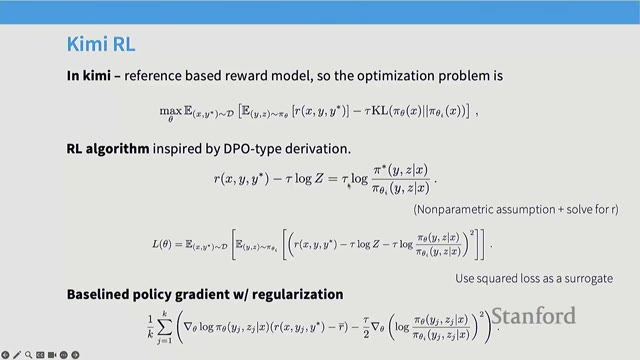
\includegraphics[width=\textwidth]{figures/fig_22_kimi_rl_algo.jpg}
\caption{Kimi K1.5：把最优策略等式做成平方损失\protect\footnotemark}
\end{figure}
\footnotetext{视频画面时间区间：01:03:30--01:04:00。}

推导路径：从 KL 正则化的奖励最大化出发，做非参数假设得到 $r(x,y) = \log \frac{\pi^*(y|x)}{\pi_{\text{ref}}(y|x)} + \log Z(x)$（与 DPO 完全一致）；但 Kimi 不代入 Bradley-Terry，而是直接说"对最优策略这个等式成立"，于是把它做成\textbf{平方损失}驱动两边靠近：

\[
\mathcal{L} = \left( r_\theta(x,y) - \log\frac{\pi_\theta(y|x)}{\pi_{\text{ref}}(y|x)} - \log Z \right)^2
\]

对它求梯度，形式上和 GRPO 非常像——策略梯度 + batch 内均值作为 baseline + 一个平方项作为正则化（替代 clip）。这说明：\textbf{只要具备策略梯度、合理 baseline、某种正则化三件套，就能得到一个能跑的 RL 算法}。

Kimi 起点的 KL 正则化目标可写为：

\[
\max_{\pi_\theta}\; \mathbb{E}_{x \sim \mathcal{D},\, y \sim \pi_\theta}\left[ r(x, y) \right] - \beta\, \mathbb{D}_{\text{KL}}\!\left( \pi_\theta(\cdot|x) \,\|\, \pi_{\text{ref}}(\cdot|x) \right)
\]

\begin{itemize}
\item 第一项：在数据集 $\mathcal{D}$ 和策略 $\pi_\theta$ 下的期望奖励
\item 第二项：KL 惩罚，防止策略漂离参考模型 $\pi_{\text{ref}}$
\item $\beta$：权衡探索与约束的系数——所有 RLHF/RLVR 算法的共同起点
\end{itemize}

\subsection{长度奖励：主动压缩 CoT}

Kimi 团队比 R1 更早意识到\textbf{推理成本}的重要性——长 CoT 极其昂贵。所以他们主动设计\textbf{长度奖励}来压缩思维链。

\begin{figure}[H]
\centering
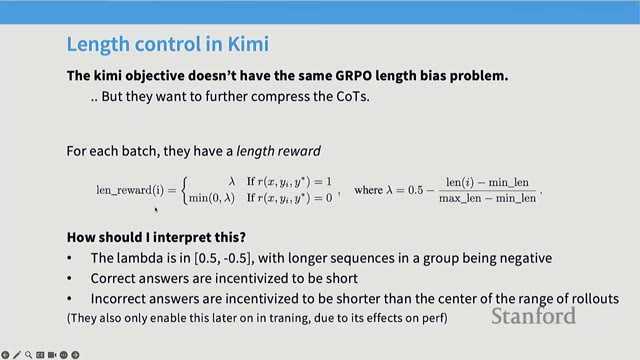
\includegraphics[width=\textwidth]{figures/fig_23_kimi_length_reward.jpg}
\caption{Kimi K1.5 长度奖励：奖励短的、惩罚长的\protect\footnotemark}
\end{figure}
\footnotetext{视频画面时间区间：01:06:45--01:07:15。}

\[
\lambda = \frac{L_{\max} - |y|}{L_{\max} - L_{\min}} - 0.5
\]

\begin{itemize}
\item $L_{\max}$、$L_{\min}$：batch 内最长、最短回答
\item $\lambda \in [-0.5, 0.5]$：越短越大
\item \textbf{答对时}：奖励 $\lambda$，激励\textbf{尽量短}
\item \textbf{答错时}：也用 $\lambda$，但压力较弱（鼓励不要太长但不强制最短）
\end{itemize}

\begin{warningbox}{长度奖励不能加得太早}
Kimi 发现：如果训练早期就加长度奖励，RL 会\textbf{停滞}——模型什么都不会做，最优策略是把 CoT 拉到最短，然后陷入局部极小再也出不来。所以正确做法是\textbf{先做一段无约束 RL，后期再加长度奖励}。
\end{warningbox}

\subsection{课程与奖励工程的其他细节}

\begin{itemize}
\item \textbf{难度标签}：人工或 LM 给数据打难度标签，按"易 $\to$ 难"顺序训练
\item \textbf{按成功率采样}：成功率 $p$ 越高的题采样权重越低；$p=1$ 的题永不采样
\item \textbf{代码奖励}：用 ground-truth 解生成测试用例
\item \textbf{数学奖励}：用一个小\textbf{奖励模型}做答案等价性判断（而非简单的 regex/string match）——令人意外的是在"可验证"场景用模型判等，但因为本质是高级字符串匹配，准确率极高
\end{itemize}

\begin{importantbox}{多个奖励如何组合？}
所有奖励（accuracy、format、length、language consistency）都是\textbf{加权求和}，权重凭经验调以最大化下游性能。format 类奖励可看作 shaping——不是终点，而是引导模型产出可用 CoT 的手段。
\end{importantbox}

\subsection{RL 基础设施}

Kimi 论文是少有的\textbf{详谈 RL 系统设计}的推理模型论文。

\begin{figure}[H]
\centering
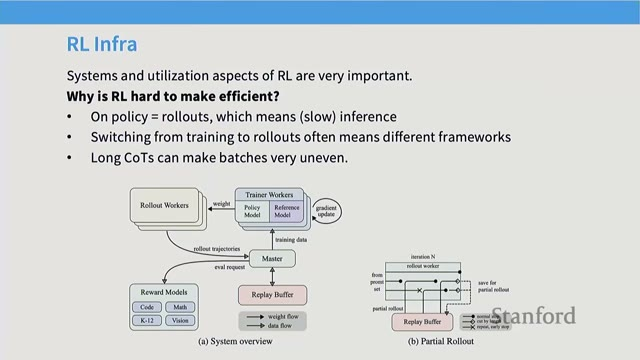
\includegraphics[width=\textwidth]{figures/fig_24_kimi_infra.jpg}
\caption{Kimi K1.5 RL 基础设施：训练 worker 与推理 worker 解耦\protect\footnotemark}
\end{figure}
\footnotetext{视频画面时间区间：01:09:30--01:10:15。}

\begin{tabular}{p{3cm}p{10cm}}
\toprule
\textbf{挑战} & \textbf{Kimi 的做法} \\
\midrule
rollout 昂贵 & 必须运行语言模型做推理，比预训练更难饱和 GPU \\
权重同步 & 训练 worker $\leftrightarrow$ 推理 worker 之间要传模型权重 \\
长 CoT & batch 长度极不均匀，需要巧妙调度 \\
vLLM & 推理用 vLLM；常"用 dummy 权重启动"，加载权重后再每轮拆毁以释放显存 \\
\bottomrule
\end{tabular}

\begin{knowledgebox}{vLLM 权重注入的工程痛点}
目前把训练侧的 RL 权重"塞进"vLLM 还非常麻烦。虽然有实验性 NCCL collective API 可直接把权重灌进去，但参数文档不全、不够成熟。当前工业界的普遍做法是"dummy 权重启动 + hack 加载 + 每轮拆 vLLM 释放显存"。Tatsu 预期一年后这套基础设施会显著成熟，A5 也会用上简化版。
\end{knowledgebox}

\subsection{Kimi 的训练曲线}

Kimi 展示了逐 RL 迭代的性能曲线：性能稳步上升，而\textbf{回答长度平台化}（不像 vanilla GRPO 那样无限增长）——这与 Dr.GRPO 的观察一致，因为 Kimi 的算法本身没有"鼓励变长"的偏差。

\section{案例研究三：Qwen3}

Qwen3 是三者中最新的，报告在课程结束前刚刚发布。它在 R1 基础上引入了若干新技巧，尤其在\textbf{推理效率}方向上有独到设计。

\subsection{整体流水线}

\begin{figure}[H]
\centering
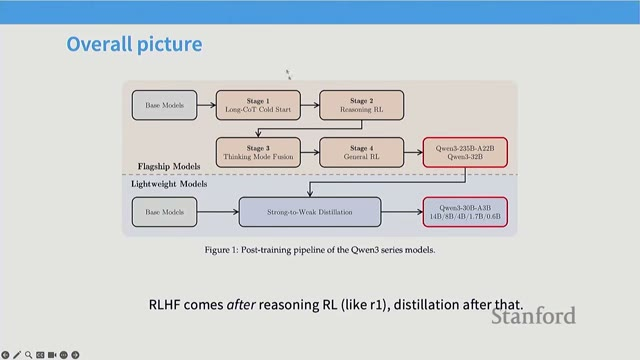
\includegraphics[width=\textwidth]{figures/fig_25_qwen3_pipeline.jpg}
\caption{Qwen3 流水线：长 CoT SFT $\to$ 推理 RL $\to$ 思维模式融合 $\to$ 通用 RL\protect\footnotemark}
\end{figure}
\footnotetext{视频画面时间区间：01:14:35--01:14:55。}

\begin{enumerate}
\item \textbf{长 CoT SFT}：手工筛选（区分"猜对"与"真会"）
\item \textbf{推理 RL}：在惊人的\textbf{3,995 个样本}上做 RL，仍获得可观增益
\item \textbf{思维模式融合（thinking mode fusion）}：Qwen3 独创
\item \textbf{通用 RL（RLHF）}：对齐一般指令
\end{enumerate}

\begin{importantbox}{3995 个样本的样本效率}
Qwen3 仅用约 4000 个 RL 样本就取得显著增益。这既说明 RLVR 的极高效率，也呼应了历史上"少量样本即可 instruction tune / 蒸馏长 CoT"的现象——但\textbf{能少样本跑通}并不等于\textbf{不能继续 scale}，背后机制目前仍不清楚。
\end{importantbox}

\subsection{思维模式融合：单模型双模式}

这是 Qwen3 最有意思的创新。其目标是\textbf{在同一个模型里同时拥有"思考模式"和"非思考模式"}：训练后对模型做 SFT，让它学会根据 \texttt{<think>} / \texttt{<no-think>} 标签决定是否展开思维链。

\begin{figure}[H]
\centering
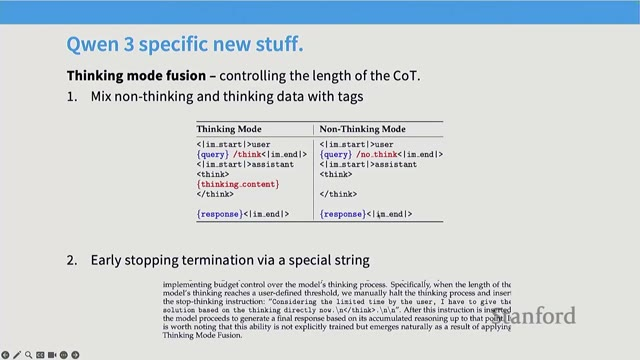
\includegraphics[width=\textwidth]{figures/fig_26_qwen3_thinking_fusion.jpg}
\caption{Qwen3 思维模式融合：think / no-think 标签 + 早停控制\protect\footnotemark}
\end{figure}
\footnotetext{视频画面时间区间：01:17:15--01:17:45。}

\begin{itemize}
\item \texttt{<think>}：正常长 CoT
\item \texttt{<no-think>}：直接给答案
\item \textbf{附加能力}：在思考过程中插入特殊字符串（如"考虑到用户的时间有限，我需要直接给出答案"）可以\textbf{优雅地提前终止思维链}，给出近乎正确的答案
\end{itemize}

\begin{practicebox}{test-time scaling 的新维度}
思维模式融合让单一模型获得精细的"思考预算"控制：思考预算设到无穷就是原思考模型；设到某阈值就提前终止，性能从满血优雅退化。这是一种非常干净的\textbf{test-time scaling 旋钮}。
\end{practicebox}

\subsection{Qwen3 的消融：推理 RL vs 通用 RL 的权衡}

\begin{figure}[H]
\centering
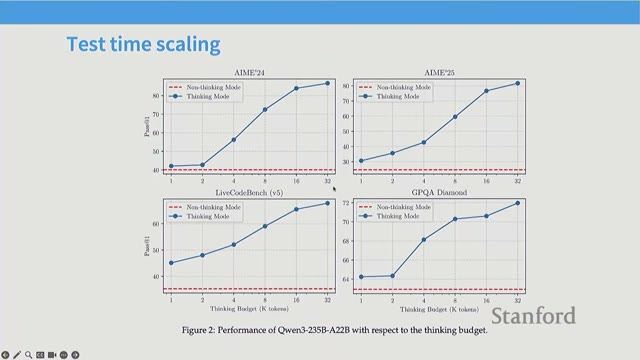
\includegraphics[width=\textwidth]{figures/fig_27_qwen3_ablation.jpg}
\caption{Qwen3 消融：推理 RL、思维融合、通用 RL 在不同任务上的影响\protect\footnotemark}
\end{figure}
\footnotetext{视频画面时间区间：01:18:30--01:19:00。}

Qwen3 给出了推理 RL、思维融合、通用 RL 三阶段在 think / no-think 两种模式下的消融：

\begin{tabular}{p{3.5cm}p{4.5cm}p{5cm}}
\toprule
\textbf{任务类型} & \textbf{推理 RL} & \textbf{通用 RL（RLHF）} \\
\midrule
通用 / 指令跟随 & think 模式下都涨 & 继续涨 \\
数学 / STEM（think） & 通用 RL \textbf{伤害}性能 & --- \\
数学 / STEM（no-think） & 通用 RL 帮助性能 & --- \\
\bottomrule
\end{tabular}

\begin{warningbox}{推理与通用能力的张力}
Qwen3 的消融揭示了一个真实存在的\textbf{权衡}：优化"通用指令跟随"和优化"数学/代码推理"在 think 模式下是冲突的——通用 RL 会拉低推理性能。如何在同一模型里同时做好两类任务，是后续模型要攻克的开放问题。
\end{warningbox}

\section{总结与展望}

\begin{figure}[H]
\centering
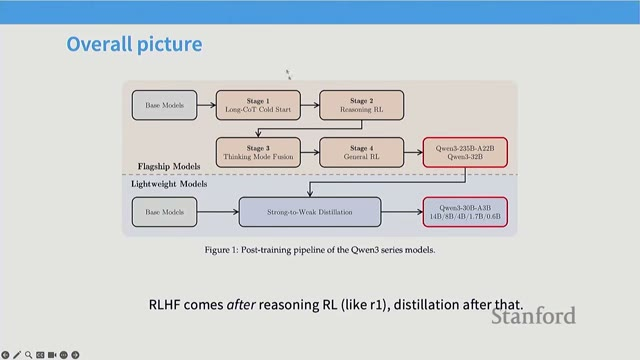
\includegraphics[width=\textwidth]{figures/fig_25_qwen3_pipeline.jpg}
\caption{三个案例的共同骨架：SFT $\to$ 推理 RL $\to$（融合）$\to$ 通用 RL\protect\footnotemark}
\end{figure}
\footnotetext{视频画面时间区间：01:14:35--01:14:55。}

\subsection{核心结论}

\begin{importantbox}{本讲的核心信息}
\begin{enumerate}
\item \textbf{RL 很强大}，但靠"对噪声成对偏好不断 hill-climb"的 RLHF 走不远
\item \textbf{解法}：选择无法 reward hacking 的领域（数学、代码），把 RL 武器全搬过来——这是 RLVR 的根本动机
\item \textbf{算法}：GRPO 极其简单——策略梯度 + 组内 baseline 即可。Dr.GRPO 进一步揭示了两个被忽视的偏差
\item \textbf{工程}：三篇论文展示了 SFT $\to$ RL $\to$ RLHF 的成功配方，以及各自的关键实现技巧
\end{enumerate}
\end{importantbox}

\subsection{三个案例的对比}

\begin{tabular}{p{2.5cm}p{3cm}p{3cm}p{3.5cm}}
\toprule
\textbf{维度} & \textbf{DeepSeek-R1} & \textbf{Kimi K1.5} & \textbf{Qwen3} \\
\midrule
RL 算法 & GRPO（clip） & 平方损失正则（类 DPO） & GRPO 变体 \\
价值模型 & 无 & 无 & 无 \\
奖励 & accuracy + format + 语言一致 & accuracy + length + 课程 & accuracy + 思维融合 \\
长度控制 & 无（被动增长） & 有（length reward） & 有（thinking budget） \\
PRM & 否 & 否 & 否 \\
搜索 & 否（MCTS 失败） & 否 & 否 \\
数据规模 & 未公开 & 未公开 & 3,995 样本 \\
\bottomrule
\end{tabular}

\begin{knowledgebox}{三者的"趋同演化"}
R1 与 Kimi K1.5 几乎同期独立完成，Qwen3 在其后吸收两者经验。三者都放弃了 PRM 与搜索、都用纯结果奖励 + 无价值模型的 RL、都遵循"SFT $\to$ 推理 RL $\to$ 通用 RL"骨架。这种趋同强烈暗示：当前推理模型的最优配方已基本收敛，差异主要在数据、长度控制与基础设施等工程层面。
\end{knowledgebox}

\subsection{贯穿全讲的几条主线}

\begin{enumerate}
\item \textbf{结果奖励胜过过程奖励与搜索}：DeepSeek 在 Math 阶段信 PRM，到 R1 放弃；MCTS 也未跑通。至今\textbf{纯结果奖励 + RL} 仍是最强基线。
\item \textbf{基线（baseline）是 RL 的灵魂}：无论是 GRPO 的组内均值、Kimi 的 batch 均值，还是 PPO 的价值函数，本质上都是降低梯度的方差。
\item \textbf{长 CoT 不是"想得更深"，可能是"目标有偏"}：Dr.GRPO 和 Kimi 的曲线都暗示，长度增长部分来自算法偏差而非内在需求。
\item \textbf{推理与通用能力的张力真实存在}：Qwen3 消融明确显示 think 模式下通用 RL 会伤害推理。这是未来模型的关键开放问题。
\item \textbf{RL 基础设施远未成熟}：vLLM 权重注入、rollout 调度、worker 解耦都还有大量工程空间。
\end{enumerate}

\begin{practicebox}{作业落地}
A5 将让你亲手实现 GRPO。你会遇到本讲提到的几乎所有细节：组内 z-score、除以标准差加 epsilon、KL 的 per-token vs per-sequence、vLLM 权重同步、外层训练循环与内层 rollout 的解耦。把这些细节跑通，你就真正理解了推理模型是如何被训练出来的。
\end{practicebox}

\end{document}
